\documentclass[conference]{IEEEtran}

\usepackage{cite}
\usepackage{amssymb}
\usepackage{amsmath}
\usepackage{mathdots}
\usepackage{graphicx}
\usepackage{comment}

\renewcommand\figurename{Fig.}



\title{\textbf{Peningkatan PageRank Berbobot untuk Menangani Kesamaan Tautan Nol}}
\author{\IEEEauthorblockN{Budi Prasetio}\\
\IEEEauthorblockA{Fakultas Teknologi Informasi\\
Institut Teknologi Batam\\
Batam, Kepulauan Riau, Indonesia\\
2022015@student.iteba.ac.id}}

\begin{document}

% Judul
\maketitle

%abstrak
\begin{abstract}
    Algoritme PageRank yang terkenal memanfaatkan struktur tautan untuk menghitung peringkat kualitas halaman. Ini pada dasarnya memberikan jumlah probabilitas yang sama ke halaman tetangga dari suatu halaman. Sebagai ekstensinya, algoritma PageRank berbobot telah diusulkan yang memberikan bobot berbeda pada tautan keluar dari sebuah halaman. Beberapa algoritma PageRank berbobot menggunakan kesamaan antar halaman sebagai bobot. Di halaman web Korea, kami menemukan bahwa terkadang memiliki nilai nol untuk kesamaan antar halaman dari halaman tetangga karena karakteristik bahasa. Makalah ini mengusulkan peningkatan algoritma PageRank berbobot yang dapat menangani kesamaan antar halaman nol tersebut. Metode yang diusulkan telah diimplementasikan menggunakan paradigma MapReduce untuk penanganan data besar, dan telah dievaluasi melalui halaman web Wikipedia bahasa Korea dan dibandingkan dengan dua metode lainnya.

\end{abstract}\hspace{10pt}
\begin{comment}
\cite{brin1998anatomy,xing2004weighted,qiao2010simrank,page1999pagerank,kumar2013pagerank,duhan2009page,najork2007comparing,kumar2011page,nemirovsky2008weighted,tyagi2012weighted,haveliwala2003topic,resnik1999semantic,schutze2008introduction,dean2008mapreduce,rajaraman2011mining,kim2007music,lee2012statistical,lee2004adaptive,lee1997hierarchical,lee2003coordinated,yoon2007end}
\end{comment}

%keyword
%\begin{IEEEkeywords}
%    PageRank; Weighted PageRank; Similarity; MapReduce; TFIDF
%\end{IEEEkeywords}
\textbf{\textit{Keywords---PageRank; Weighted PageRank; Similarity; MapReduce; TFIDF}}
%pendahuluan
\section{Introduction}
Saat ini, ketika orang ingin mengetahui sesuatu, banyak dari mereka mencoba mencarinya di Internet. Mereka akan kewalahan jika terlalu banyak halaman yang diberikan sebagai halaman yang relevan dalam pencarian web. Dalam information retrieval (IR), pemeringkatan menjadi salah satu isu krusial. Untuk memilah yang berpengaruh di antara halaman yang dicari, berbagai algoritma peringkat telah diusulkan. \cite{brin1998anatomy,xing2004weighted,qiao2010simrank,page1999pagerank,kumar2013pagerank,duhan2009page,najork2007comparing,kumar2011page,nemirovsky2008weighted,tyagi2012weighted,haveliwala2003topic}

PageRank 
\cite{brin1998anatomy}
adalah salah satu algoritma peringkat terkenal yang menggunakan struktur link Web. Ini mengasumsikan bahwa seorang peselancar berjalan secara acak di atas halaman web dan mencoba untuk menentukan distribusi statis dari peselancar. Dengan metafora penderitaan acak, semakin banyak tautan yang dimiliki halaman, semakin tinggi peringkatnya. Di PageRank, penderitaan membuat jalan acak ke halaman tetangga dengan probabilitas yang sama.
Kadang-kadang probabilitas yang sama ini tampaknya tidak masuk akal karena beberapa tautan terhubung ke halaman tetangga yang jauh lebih penting.\\

Untuk mengatasi situasi ini, algoritma PageRank berbobot
\cite{xing2004weighted,qiao2010simrank,kumar2011page}
telah diusulkan. Mereka memperhitungkan baik distribusi jumlah in-link untuk node tetangga, the jumlah kunjungan ke halaman tetangga, atau antar halaman kesamaan. Masing-masing memiliki pro dan kontra. Pembobotan berdasarkan kesamaan antar halaman terdengar baik dalam melayani peringkat berbasis konten.
Kami telah mencoba pembobotan berbasis kesamaan antar halaman
Algoritma PageRank ke halaman Wikipedia bahasa Korea. Untuk
menghitung kesamaan antar halaman, kami menggunakan vektor
model\cite{schutze2008introduction}. Untuk mendapatkan representasi vektor untuk halaman, pertama-tama kita
melakukan analisis morfologi untuk mengekstrak kata-kata.
Berbeda dengan bahasa barat, kata benda dalam bahasa Korea paling banyak menyampaikan
informasi yang berarti. Karena karakteristik bahasa,
kata benda diekstraksi untuk mengidentifikasi kata kunci. Kata kunci
diidentifikasi menggunakan istilah frekuensi dan dokumen terbalik
informasi frekuensi. Dengan kata kunci, vektor
representasi untuk halaman diperoleh. Kemudian, itu terjadi pada
memiliki kesamaan nol ketika kesamaan antar halaman dihitung
menggunakan produk dalam dari vektor tersebut. Ini sangat canggung untuk halaman tetangga tidak memiliki kesamaan. makalah ini adalah terkait dengan peningkatan pada PageRank berbobot berbasis kesamaan antar halaman untuk menangani kasus dengan nol link kesamaan.\\

Sisa makalah ini disusun sebagai berikut: Bagian
II menyajikan PageRank dan variannya lebih detail.
Bagian III memperkenalkan peningkatan pada pembobotan
PageRank, dan Bagian IV menunjukkan beberapa hasil eksperimen untuk
metode yang diusulkan. Kami menarik kesimpulan di Bagian V.
%relate works
\section{Related works}
\subsection{PageRank Algorithm}
PageRank\cite{brin1998anatomy} adalah algoritma perbatasan yang memberi peringkat halaman
dengan mengacu pada struktur link Web. suguhan PageRank
halaman sebagai node dan hyperlink sebagai tepi grafik. Setiap simpul
memiliki nilai Rank sendiri dan mendistribusikannya secara merata ke tetangganya.
Distribusi berulang tanpa batas sampai semua nilai peringkat adalah
konvergen. Distribusi stasioner dari Ranks adalah
dianggap sebagai skor Peringkat akhir halaman. Untuk mencegah
peningkatan tak terbatas dalam nilai Peringkat, itu dibatasi untuk jumlah
dari semua Peringkat menjadi 1, dan juga untuk setiap nilai Peringkat menjadi tidak
lebih besar dari 1.Nilai peringkat dari simpul j dihitung sebagai
berikut:

\begin{equation}
    \begin{gathered}
    r_{j}=\sum_{i_{\text {out }}} \frac{r_{i}}{L_{\text {out }}(i)} \\
    \end{gathered}
    \end{equation}
    \begin{equation}
        \begin{gathered}
        \sum r_{i}=1
        \end{gathered}
        \end{equation}

dimana ${L_\text{out}}$ adalah jumlah out-link dari node $i$.Setiap simpul $i$ mendistribusikan skor peringkatnya $r_i$ secara merata simpul tetangganya $j$.
SEBUAH
node $j$ mengumpulkan semua skor Rank yang dikirimkan dari tetangga
node dan ambil jumlah mereka sebagai skor Peringkat baru $r_j$. Peringkat ini
proses distribusi dapat dinyatakan dengan kedekatan stokastik
matriks $M$ dan vektor pangkat $r$. Matriks $M$ adalah tetangganya
matriks untuk web yang mengkodekan hubungan lingkungan
antara halaman dan distribusi stasioner nilai Peringkat. Baru
Nilai peringkat $r^{(t+1)}$ dihitung sebagai berikut:
\begin{equation}
    r^{(t+1)}=\mathrm{Mr}^{(t)}
    \end{equation}

    di mana $t + 1$ adalah langkah selanjutnya dari $t$.Ketika semua nilai peringkat adalah
    konvergen, $r^{(t+1)}$ sangat mirip dengan $r^{(t)}$. Di sini, konvergen
    rsesuai dengan vektor eigen dengan nilai eigen 1 untuk matriks $M$.
\subsection{WeightedPageRank Algorithms}
Surfers sebenarnya tidak melakukan random walk seperti di PageRank.
Untuk mengakomodasi karakteristik perilaku seperti itu, pembobotan
Algoritma PageRank telah diusulkan yang memungkinkan penderitaan
untuk membuat transisi probabilistik yang tidak merata ke tetangga
halaman.\cite{xing2004weighted,qiao2010simrank,kumar2011page}\\

\subsubsection{Weighted PageRank Based on the number of in-links of neighboring pages}
\noindent

Xing dan Ghorbani\cite{xing2004weighted} mengusulkan PageRank
algoritma yang memberikan lebih banyak porsi Rank ke tetangga
halaman dengan lebih banyak tautan. Ya tidak cukup
mencerminkan perilaku peselancar yang sebenarnya, karena hanya
informasi struktur topologi digunakan.\\


\subsubsection{Weighted PageRank based on Similarity Measure}
\noindent

Qiaoet al.\cite{qiao2010simrank} menyarankan varian PageRank berbobot
algoritma, yang disebut SimRank, yang mendistribusikan nilai Rank di
porsi kesamaan antar halaman. Untuk menerapkan metode,
semua kesamaan halaman berpasangan perlu dihitung lebih awal.
Secara komputasi mahal untuk menerapkan metode ini untuk skala besar
volume halaman. Oleh karena itu untuk menerapkan metode, perlu
infrastruktur komputasi paralel terdistribusi seperti Hadoop
Pengurangan Peta\cite{dean2008mapreduce}.\\

\subsubsection{Weighted PageRank based on visits of links}
\noindent

Kumaret al.\cite{kumar2011page} memperkenalkan algoritma PageRank 
berbobot di mana node mendistribusikan lebih banyak nilai Rank ke yang keluar
tautan yang lebih sering dikunjungi oleh pengguna. Ini
algoritme memerlukan data klik tautan di seluruh
Web. Oleh karena itu, sangat ideal, tetapi tidak mudah untuk menerapkannya pada
skala web.\\

\subsection{Hub and Authorities Algorithm}
Najork\cite{najork2007comparing} mengambil pendekatan yang agak berbeda dari PageRank
dan mengusulkan algoritma peringkat yang disebut HITS (hyperlink
pencarian topik yang diinduksi). Sementara PageRank mengasumsikan gagasan satu dimensi tentang pentingnya halaman, tampilan HITS
halaman penting memiliki dua rasa penting.\cite{rajaraman2011mining} Itu
algoritma karena itu memberikan dua skor untuk setiap halaman. Yakin
halaman sangat berharga karena memberikan informasi tentang
tema. Halaman-halaman ini disebut otoritas. halaman lainnya adalah
berharga karena mereka memberi tahu Anda ke mana harus pergi untuk mencari tahu
topik itu. Halaman-halaman ini disebut hub. Algoritma mendefinisikan
dua konsep secara rekursif. Sebuah halaman adalah
dianggap sebagai hub yang baik jika terhubung dengan otoritas yang baik. Sebuah halaman adalah
dianggap sebagai otoritas yang baik jika dihubungkan dengan hub yang baik.\cite{rajaraman2011mining}

\subsection{Distributed and Parallel Computing}
Pengambilan informasi dari repositori data besar, seperti
Web dan penyimpanan data besar membutuhkan infrastruktur komputasi yang
menyimpan dan memproses data tersebut. Kita dapat menggunakan salah satu dari
sistem superkomputer atau komputasi terdistribusi dan paralel
sistem.\\

Hadoop\cite{dean2008mapreduce} adalah infrastruktur komputasi yang baik yang dapat
ditetapkan dalam biaya ekonomi. Ini adalah proyek Apache untuk
platform komputasi terdistribusi yang menyediakan seperti
sistem file terdistribusi yang disebut HDFS (Hadoop Distributed File
System) dan kerangka kerja komputasi paralel terdistribusi yang disebut
Kurangi Peta. Kerangka kerja MapReduce mengatur pekerjaan ke dalam Peta
tugas dan Mengurangi tugas. Data input dipartisi dan diproses
oleh proses Peta, dan hasil pemrosesannya dibentuk menjadi
pasangan nilai kunci. Hasil tugas peta dikocok menjadi Reduce
tugas sesuai dengan kunci mereka. Kurangi proses agregat
nilai dengan kunci yang sama, untuk mendapatkan hasil akhir. Ini
kerangka kerja komputasi memungkinkan kita untuk menangani beban berat
komputasi seperti komputasi kesamaan halaman berpasangan.
\section{The Proposed Algorithm}
PageRank berbobot berbasis kesamaan antar halaman
pada kesamaan tidak dapat menangani situasi yang antar halaman
kesamaannya adalah 0. Untuk menghadapi situasi ini, kami mengusulkan a
metode untuk menjaga kesamaan antar halaman nol dan untuk menyesuaikan
bobot untuk distribusi nilai Rank.\\

Ekstraksi kata kunci berbasis kata benda seperti di halaman Korea
terkadang menemukan kata kunci umum di antara halaman yang ditautkan.
Terlepas dari gagasan yang melekat tentang kesamaan antar halaman untuk memperkirakan
frekuensi traversal tautan, situasi nol-kesamaan menghalangi
penerapan algoritma PageRank berbobot.\\

Untuk meningkatkan penerapan PageRank berbobot, kami
mengusulkan metode untuk menjamin beberapa bobot minimum dan
menyesuaikan bobot. PageRank berbobot yang diusulkan berfungsi sebagai
berikut, yang pada dasarnya berperilaku dengan cara yang sama seperti Qiao
algoritme et al.\cite{qiao2010simrank}\\

Berdasarkan ukuran kemiripan, bobot ${w_{ij}}$ pada node $i$ ke $j$ dihitung sebagai berikut:
\begin{equation}
    w_{i j}=\frac{s_{i j}}{\sum_{k \in L_{\text {out }}(i)} s_{k}}
    \end{equation}

    di mana ${s_{ij}}$ adalah kesamaan antara halaman $i$ dan $j$ dan ${L_{\text {out }}(i)}$ menunjukkan halaman yang ditunjuk oleh halaman $i$.\\

    Nilai Peringkat $r_j$ dari halaman $j$ diperbarui, hingga semua peringkat
nilai konvergen, sebagai berikut:
\begin{equation}
    r_{j}=\sum{i \in L_{i n}(j)} \beta w_{i j} r_{i}+(1-\beta) \frac{1}{N}
    \end{equation}

    di mana $\beta$ menunjukkan tingkat teleportasi seperti di PageRank,
    ${L_{ln}(j)}$ adalah halaman yang mengarah ke halaman $j$, dan $N$ adalah totalnya jumlah halaman.

    Untuk mengukur kesamaan antar halaman, kami menggunakan cosinus
    jarak antara vektor kata kunci yang elemennya adalah
    Nilai TFIDF dari lemma. Lemma diekstraksi dari
    Halaman Korea menggunakan penganalisa morfologi Korea. TF
    (Frekuensi Istilah) adalah frekuensi lemma dalam satu halaman, dan
    IDF (Frekuensi dokumen terbalik) adalah frekuensi halaman
    mengandung lemma.\cite{schutze2008introduction} Untuk kata kunci di halaman, TFIDF-nya
    dihitung sebagai berikut:
    \begin{equation}
        \text { TFIDF }=\frac{T F}{\log \left(\frac{D F}{N}\right)}
        \end{equation}

        Selanjutnya, kesamaan ${S_{ij}}$ antara halaman $i$ dan $j$ dihitung
        dengan jarak cosinus antara vektor kata kunci TFIDF nilai:
        \begin{equation}
            s_{i j}=\frac{K_{i} \cdot K_{j}}{\left|K_{i} \| K_{j}\right|}
            \end{equation}
            di mana $K_i$adalah vektor kata kunci halaman $i$.\\

            Menggunakan kesamaan dari Persamaan (7), bobot dihitung sebagai:
Persamaan (4). Namun, itu tidak mempertimbangkan situasi bahwa kesamaan antar halaman adalah nol. Oleh karena itu, kami mengusulkan suatu algoritma, yang
menanganinya dengan mengalokasikan kesamaan minimum ke tautan ke
halaman dengan kesamaan nol.
\begin{equation}
    \rho \frac{\min \left(s_{i j}\right)}{\sum_{L_{i n}(l)} s_{i k}}=\alpha(1-\rho) Z R
    \end{equation}
    di mana $\rho$ adalah parameter yang disediakan pengguna untuk kesamaan nol,
dan $ZR$ adalah jumlah tautan kesamaan bukan nol.\\

Persamaan (8) dikembangkan untuk membuat kesamaan yang disesuaikan dengan
bobot kesamaan nol lebih kecil dari kesamaan bukan nol
nilai-nilai. ditentukan menurut Persamaan(8), dimana
kesamaan minimum dikendalikan oleh $\alpha$. Bersama dengan yang disesuaikan
kesamaan baru, bobotnya hanya perlu dihitung ulang sebagai
biasa. Pada akhirnya, nilai peringkat ditentukan seperti pada
algoritma PageRank berbobot dengan Persamaan (4).
    \section{Experiments}
    Untuk mengevaluasi kinerjanya, kami menerapkan
    metode yang diusulkan untuk menentukan peringkat halaman web dalam bahasa Korea
    Wikipedia. Kami telah mengumpulkan sekitar 300.000 halaman dari
    Wikipedia bahasa Korea. Gambar 1 menunjukkan sistem percobaan
    Arsitektur\\

    Seluruh halaman dari ko.wikipedia.org telah dirayapi dan
disimpan ke dalam Hadoop HDFS. Halaman diurai menggunakan a
Penganalisa morfologi Korea untuk mengekstrak lemma. hadoop
Program MapReduce dikembangkan untuk menghitung kejadian
dari kata-kata di halaman. Berdasarkan data jumlah kata,
TFIDF untuk lemma setiap halaman dihitung untuk
menentukan kata kunci, dan vektor kata kunci dibuat untuk
setiap halaman. Vektor kata kunci dinyatakan dengan
dihitung nilai TFIDF. Kesamaan antara tetangga
halaman dihitung menggunakan jarak cosinus. Akhirnya,
nilai peringkat ditentukan oleh Persamaan (4) menggunakan bobot yang dihitung.\\

\begin{figure}[ht]
    \centering
    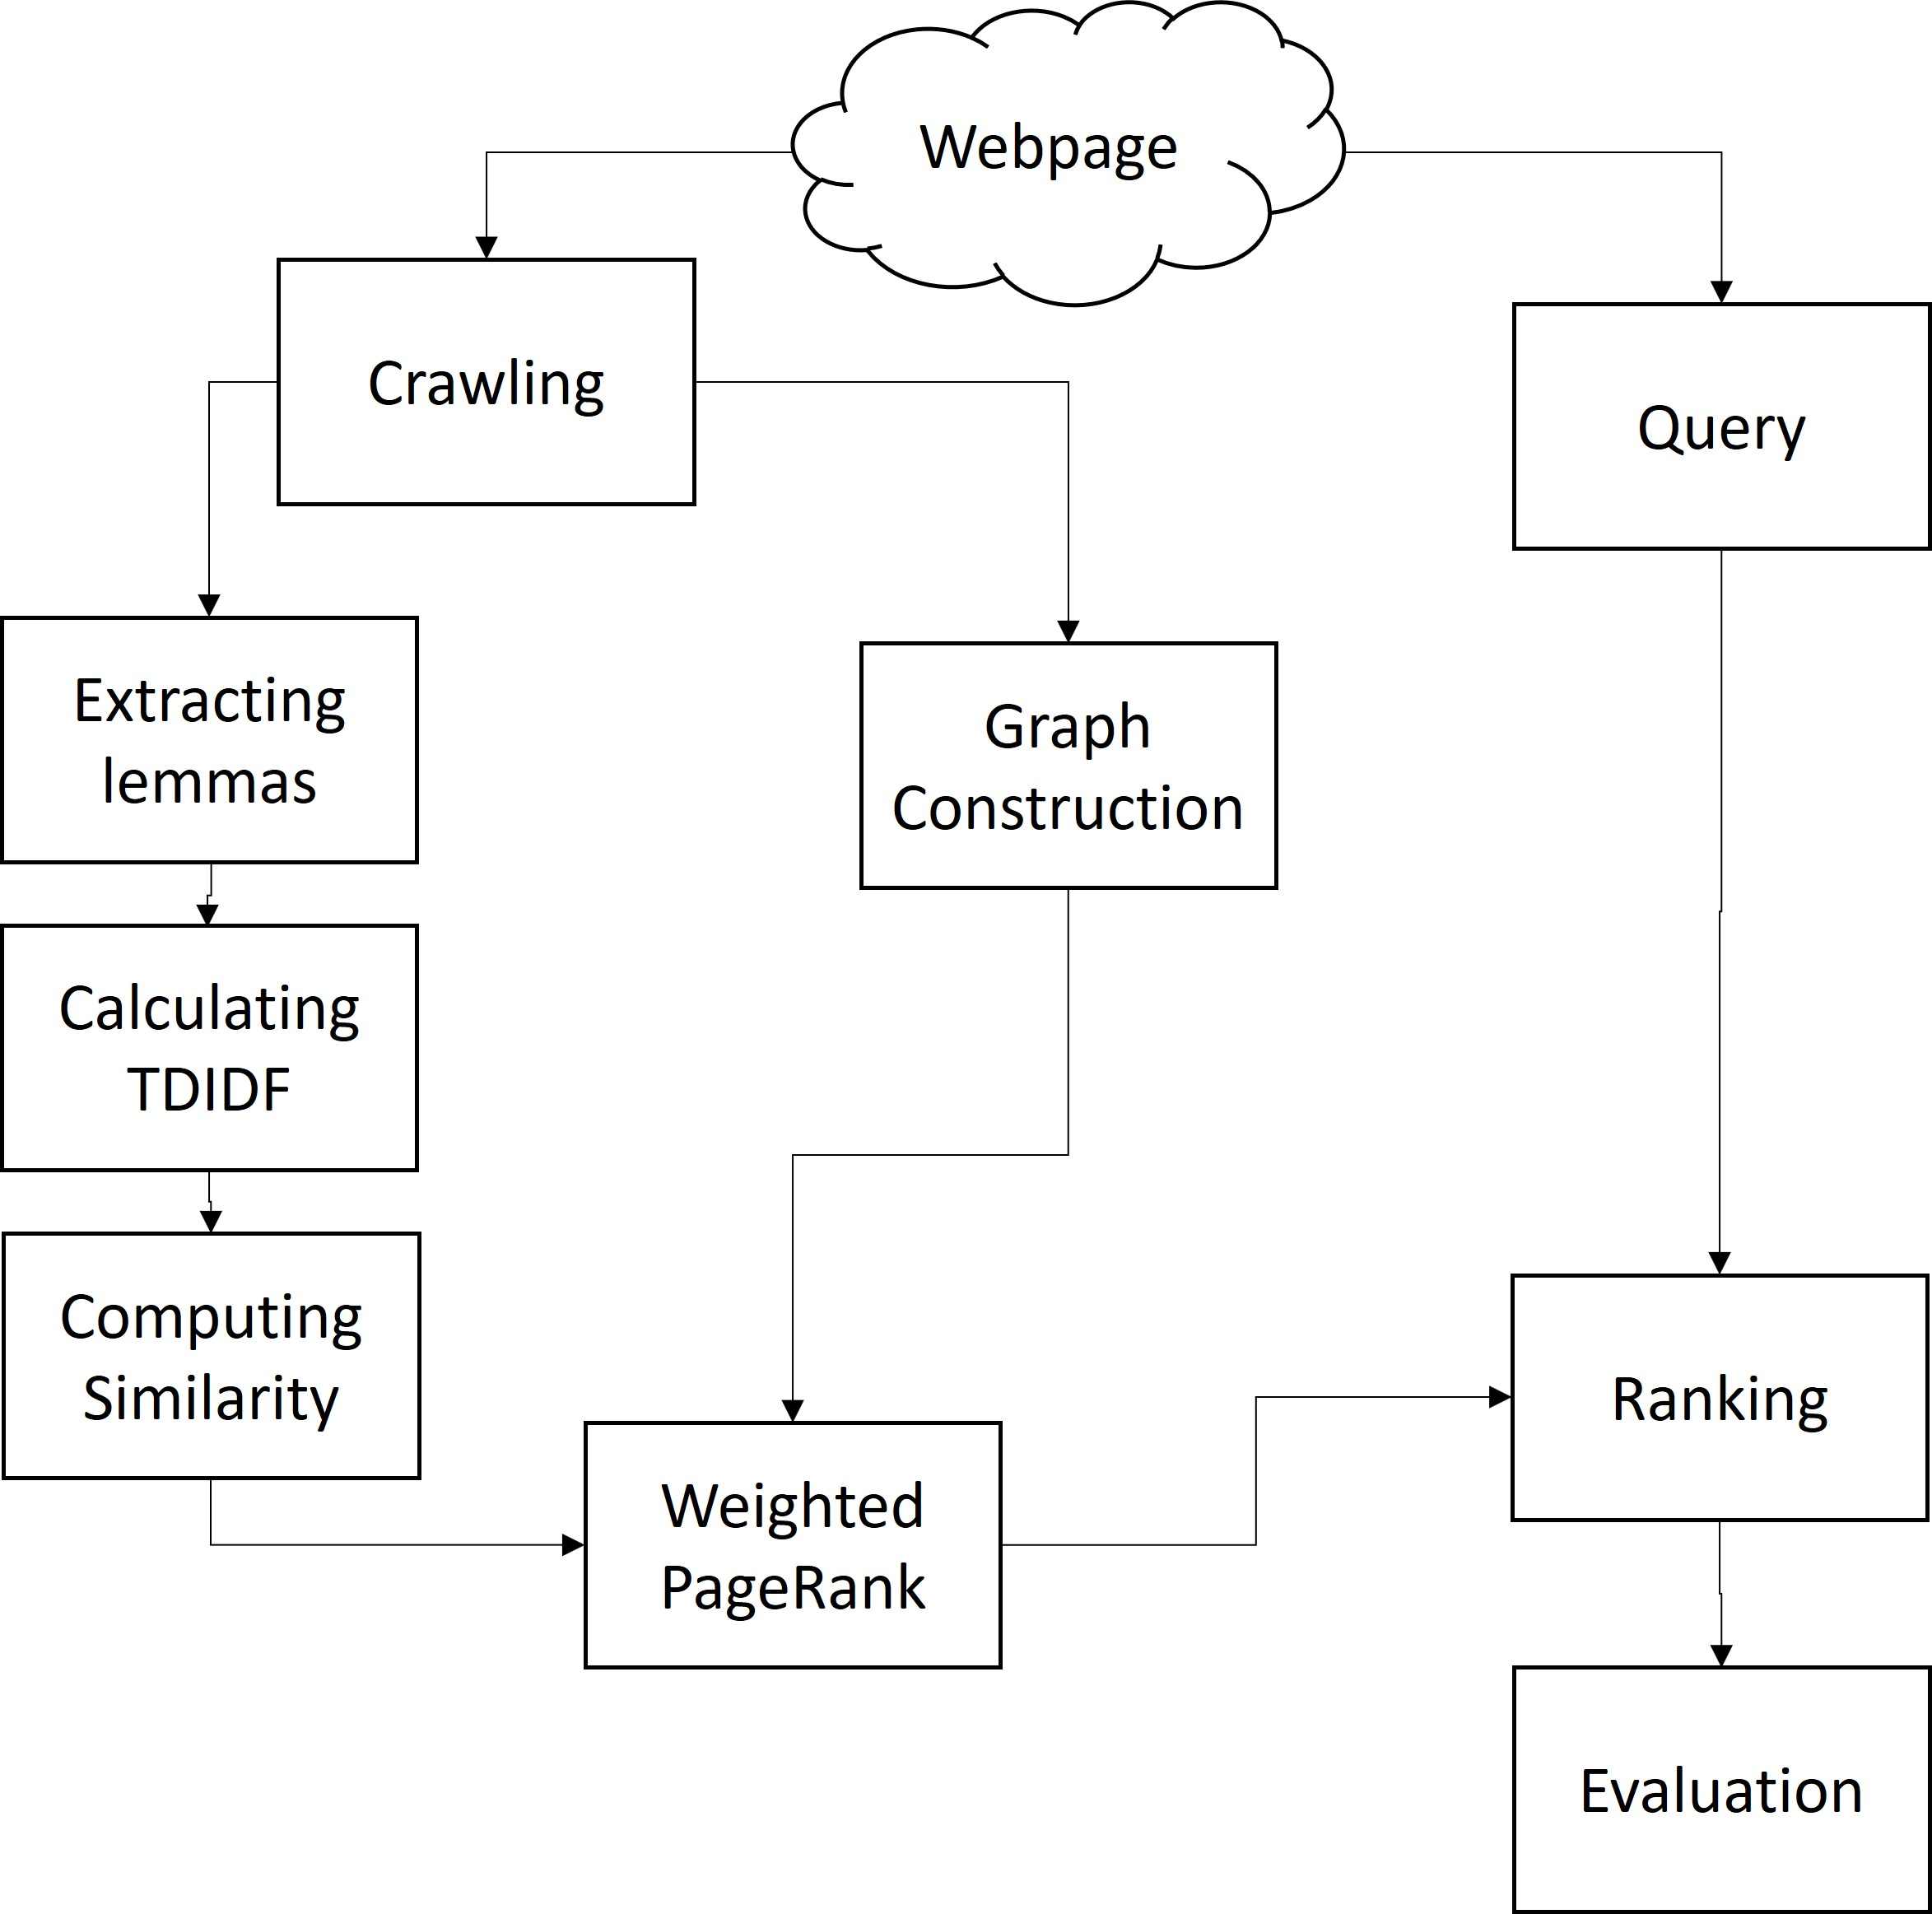
\includegraphics[width=0.4\textwidth]{pic2.jpg}
    \caption{Experiment System Architecture}
    \label{fig:logo}
    \end{figure}
Dalam percobaan, kami menggunakan cluster Hadoop dari 5 node untuk
menangani volume data yang besar. Semua tugas yang diusulkan
metode telah diimplementasikan dalam program MapReduce. Kami
melakukan percobaan 10 kali untuk dipilih secara acak 10
kata kunci dari Wikipedia dan menemukan halaman yang mengandung
kata kueri dan mengurutkannya menurut urutan menurun
dari nilai peringkat mereka. Kemudian kami memilih 20 halaman teratas dan
dievaluasi relevansinya dengan 5 skala level. Kami menghitung
Keuntungan Kumulatif Diskon yang Dinormalisasi (NDCG)\cite{schutze2008introduction} untuk
20 halaman teratas untuk setiap kueri. NDCG adalah metrik evaluasi
yang digunakan untuk mengevaluasi kinerja mesin pencari web.
Ini memberikan nilai dari 0,0 hingga 1,0, dan nilai 1,0 adalah yang ideal
peringkat entitas. Halaman kebenaran dasar untuk pertanyaan adalah
ditentukan dengan memilih halaman tautan keluar dari halaman kueri di
penurunan urutan kesamaan.\\

Gambar 2 menunjukkan hasil percobaan untuk aslinya
PageRank, Qias dkk.[3] metode dan metode yang diusulkan
dalam hal NDCG. Diamati bahwa metode yang diusulkan
telah memberikan peningkatan sekitar 2\% rata-rata selama
PageRank asli. Selama Qias et al.\cite{qiao2010simrank}, yang diusulkan
metode meningkat di NDCG sekitar 1,3\%.\\

Dari percobaan, kami mengamati bahwa yang diusulkan
metode menghasilkan hasil yang sedikit lebih baik secara rata-rata
dibandingkan dengan metode lainnya.
\begin{figure}[ht]
    \centering
    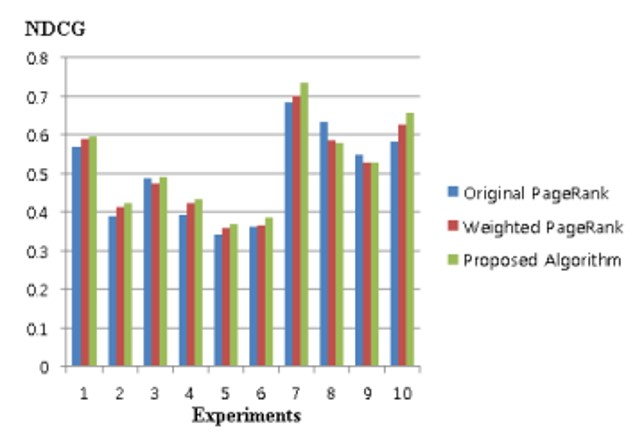
\includegraphics[width=0.4\textwidth]{pic1.jpg}
    \caption{Comparison of the original PageRank and the proposed Algorithm}
    \label{fig:logo1}
    \end{figure}

\section{Conclusion}
Dalam penelitian ini, kami menganalisis perilaku tertimbang
algoritma PageRank dan mengidentifikasi bahwa kesamaan
algoritma PageRank berbobot berbasis tidak dapat bekerja dengan baik di
beberapa situasi, terutama, ketika kata kunci kata benda adalah
diekstraksi dari halaman Korea untuk perhitungan kesamaan. baru
varian dari algoritma PageRank berbobot diusulkan untuk
menangani nol kesamaan antar halaman. Untuk volume data yang besar
pemrosesan, algoritma yang diusulkan diimplementasikan dalam
Program MapReduce dan set data eksperimental adalah
diproses pada cluster Hadoop dari 5 node. yang diusulkan
algoritma telah diterapkan ke Wikipedia Korea untuk
evaluasi kinerja. Dalam percobaan, kami menerapkan
tiga algoritma: PageRank asli, Qias et al.'s
PageRank berbobot\cite{qiao2010simrank}, dan metode yang diusulkan. Dari
percobaan kami telah mengamati metode yang diusulkan tercapai
beberapa peningkatan dalam hal NDCG dibandingkan yang dibandingkan
metode.

\section*{ACKNOWLEDGMENT}
Penelitian ini didukung oleh MSIP (Kementerian
Sains, ICT dan Perencanaan Masa Depan), Korea, di bawah the
Dukungan ITRC (Pusat Penelitian Teknologi Informasi)
program (NIPA-2013-H0301-13-4009) diawasi oleh
NIPA (Badan Promosi Industri TI Nasional)

\bibliographystyle{IEEEtran}
\bibliography{references}

\end{document}